\section{Emitter EPS}
\label{emitter_EPS}

The following section will give the final design of the emitter EPS and the reasoning behind it.
Each part of the subsystem will be dealt with seperately. The first part are the solar panels.
\\\\
In the mid term report the conclusion of the trade-off was that thin sheet solar panels made with CIGS-cells would be the best option. However, ultimately triple junction GaAs cells were chosen. This was because of two reasons. First, the triple-junction cells have a much higher efficiency than the CIGS cells which means that the solar panels will have a much smaller area. Our low orbit has the consequence that the drag due to the atmosphere will be quite high. Therefore, anything that will decrease drag will be a good design option. The second reason for choosing the triple junction cells is also because of the lower solar panel area. A lower area will be beneficial for out ballistic drag coefficient. This helps us in keeping our constellation of satellites in the correct position with respect to each other.
\\\\
Power is transferred from the solar panels to the bus using a direct-energy-transfer shunt regulator. This system extracts the necessary amount of power from the solar panels and shunts away any excess power. The power is then sent towards a DC-DC convertor. This device converts an input direct current coltage to another, higher or lower, direct current voltage. The converted power is then sent to the individual loads or to the battery for charging. The chosen convertor was developed by Clyde Space Ltd \cite{ClydeSpace}. It has one input that is converted in to 7 different outputs at different voltages. This implies a regulated bus. An unregulated bus, with converters at each subsystem that requires power, is also possible but because there are more parts required the simpler, one convertor option was chosen.
\\\\
The solar panels well be continously turned so that the cosine loss is at a minimum at all times. This will help to keep the panel area as low as possible. The result is that the weight, area and cost will also be kept as low as possible. A custom made driver was designed using a stepper motor, a gearhead and a controller unit, all from Faulhaber GMBH $\&$ CO \cite{faulhaber}. But the driver can only rotate the solar panels about one axis. Therefore the panels wilt still not be fully illuminated at all times. During initial design, an average value for the cosine loss was assumed. To verify this value, the satellite was modeled using the Satellite ToolKit software program. During preliminary design, the required power for the subsystems was 102.12 W for the emitter. Adding a safety margin of $15\%$ this would mean that the power system would need 6.2 W to operate. This brings the total power requirement up to 122.638 W. The power budget per subsystem can be seen in \ref{tab:emitterPowerBudget}. This required a solar panel area of about 1.4 square meters. The STK program calculated that solar panels of that size would yield an average value of 147W. This is more than the required power, so the assumed value for the cosine loss was good, considering that at this stage all margins should still be quite large.  Figure \ref{fig:powersim} shows the simulated power generation for one typical day. As can be seen, there are 15 orbits every day with eclipse periods in betweeen where there is no power generations.

\begin{table}
\centering
\begin{tabular}{cc}
\toprule
Subsystem & Power requirement [W]\\
\midrule
Communications & 58\\
Navigation & 1.12\\
OEP & 40\\
ORP & 0.2\\
ADCS & 2.8\\
\midrule
Total & 102.12\\
Safety margin of $15\%$ & 15.318\\
EPS & 6.2\\
\midrule
\midrule
Grand Total & 123.638\\
\bottomrule
\end{tabular}
\caption{Emitter power budget}
\label{tab:emitterPowerBudget}
\end{table}

\begin{figure}[H!]
\centering
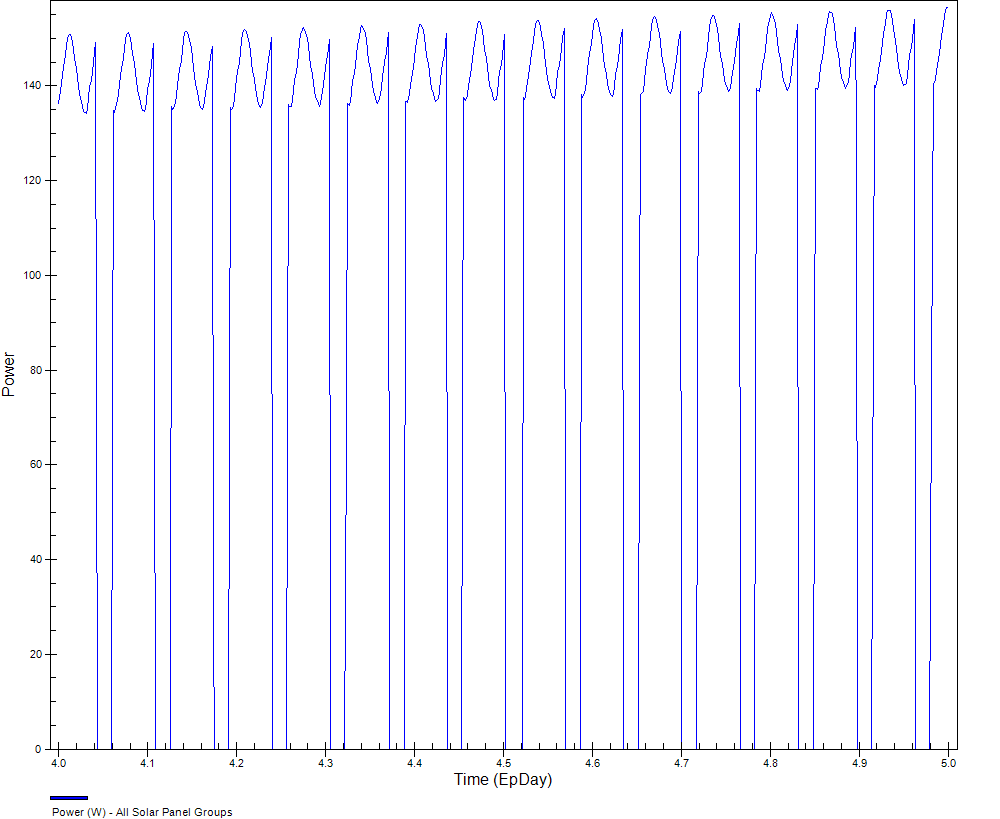
\includegraphics{chapters/img/powerSim.png}
\caption{Simulated power generation of emitter satellite solar panels}
\label{fig:powersim}
\end{figure}

During launch, the solar panels are held down by Dyneema wire bundles. These cables are cut by the DutchSpace thermal knife concept \cite{dutchspace}. The 'cutting' of the cables works as follows: electrical power is dissipated through a resistor on a ceramic plate (the blade of the knife). The resulting heat dissolves the links between the molecules in the aramid material of the cable. After about thirty seconds, the cables have been cut through. This system offers some advantages over deployment mechanisms that use pyrotechnic shocks. Because the tension in the cables lessens gradually, there are no high shocks during the release of the solar panels. Also, the thermal knife can be used multiple times, so it can be tested on the ground before it is used on a satellite. Thirdly, because there are no moving components, the system is less complex and has a higher reliability.
\\\\
For the deployment of the panels from their stowed position during launch to their fully deployed position when in orbit the smart memory alloy technique is used. In this concept, the SMA strips are heat treated in the deployed (hot) configuration and joined at the ends by metallic structural fittings. In the martensitic (cold) state, the hinge is manually buckled and folded into the stowed configuration. Application of heat via internally bonded, flexible nichrome heaters transforms the SMA into the austenitic (hot) state and causes the hinge deploy. Once deployed power is turned off and the SMA is allowed to cool back to the low temperature martensitic phase. Although the martensite phase is softer than the high temperature austenite phase, the very efficient section geometry in the deployed configuration allows the martensitic SMA hinge to support the lightweight solar array sections.
\\ \\
An important part of the EPS are the batteries. Recently, lithium-ion batteries have been developed and tested with the result that they are space qualified for LEO missions \cite{LEO_li_ion}. There are three batteries, each one made up of two modules connected in parallel which each consist of 7 lithium-ion cells connected in series. This gives an output voltage of 28V at a capacity of six ampere-hours per battery.
The amount of wiring was determined from SMAD and was based on the dry mass of the satellite.
\\ \\
Table \ref{tab:EPS_detailsEm} shows the dimensions, weight and power usage of each part of the emitter satellite's electrical power system. The losses of the solar panels and batteries are considered in their design, therefore their power use is listed as zero in this table.


\begin{table}[H!]
\centering
\begin{tabular}{cccccc}
\toprule
Part & \multicolumn{3}{c}{Dimensions [mm]} & Weight [g] & Power usage [W]\\ 
\midrule
 & Length & Width & Height & & \\ 
 Drivers (2) & 30 & 6 & 60 & 21.4 & 1 \\ 
 SMA Deployment (2) & 120 & 50 & 10 & 120 & 4* \\ 
 Battery (3) & 168 & 102 & 10 & 1000 & 0 \\ 
 Convertor & 95 & 60 & 17 & 80 & 1.5 \\ 
 Shunt regulator (2) & 2.8 & 2.6 & 1.05 & 0.1 & 0.5 \\ 
 Thermal knife (2) & 60 & 50 & 38 & 280 & 15**  \\
 Wiring & - & - & - & 430 & 1.7 \\ 
 Solar panels (2) & 1200 & 600 & 5.538 & 723.5 & 0 \\
 \midrule
 TOTAL & - & - & - & 5800 & 6.2***  \\ 
\bottomrule
 \multicolumn{6}{l}{* for 4 minutes} \\
 \multicolumn{6}{l}{** for 60 seconds} \\
 \multicolumn{6}{l}{*** continuous power usage only} \\
\end{tabular}
\caption{EPS subpart details for receiver satellites}
\label{tab:EPS_detailsEm}
\end{table}

The architecture of the power system is show in figure \ref{fig:emitter_block}. The power from the solar panels is transferred to the dc-dc convertor. There part of it is sent to charge the batteries and part is sent to power the payload. During eclipse periods, the power is sent from the batteries to the payload via the convertor.

\begin{figure}[H!]
\centering
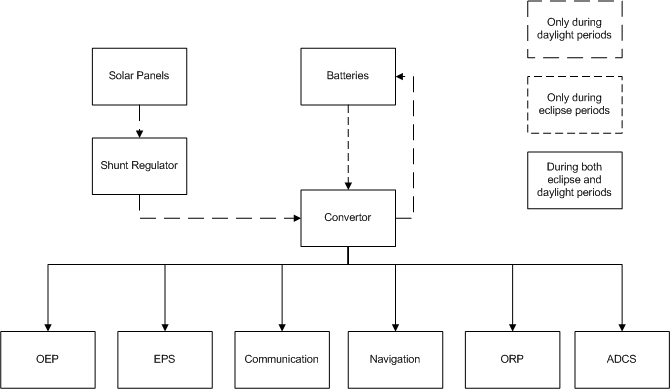
\includegraphics{chapters/img/EPS_emitter_block_diagram.png}
\caption{Electrical block diagram of the emitter}
\label{fig:emitter_block}
\end{figure}
